\section{Documents}\label{sec:fa_documents}

\begin{figure}[H]
  \centering
  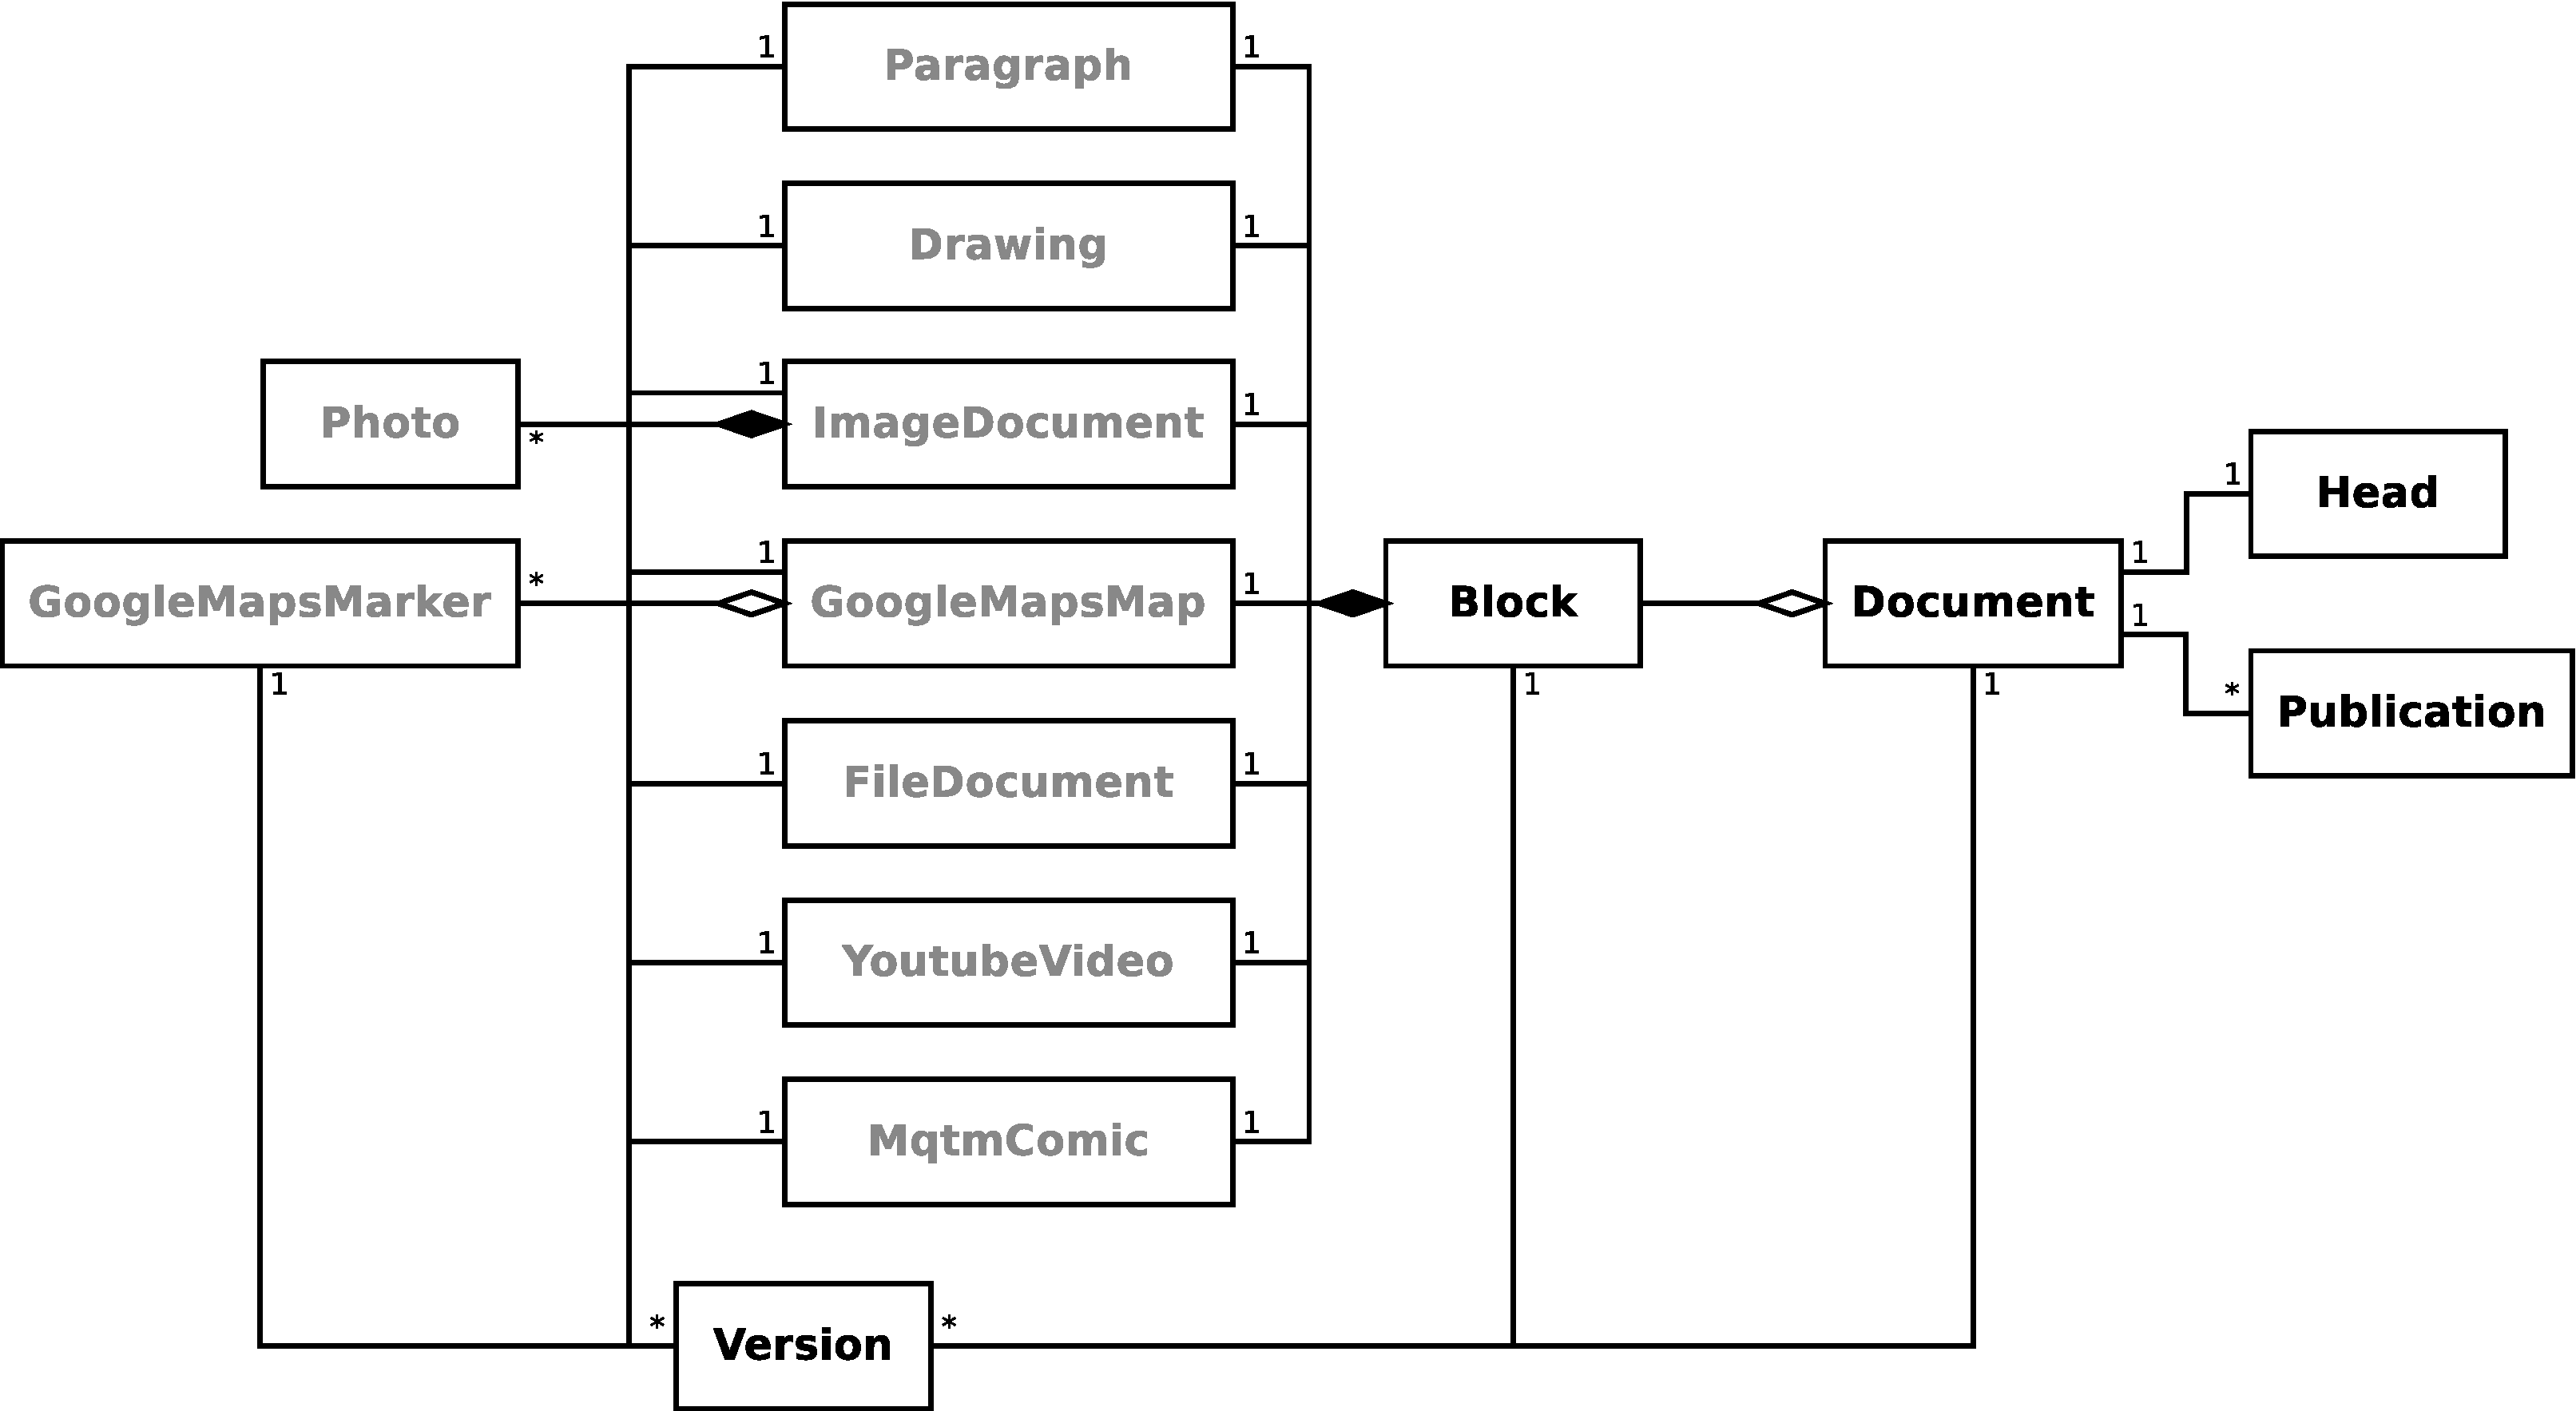
\includegraphics[width=165mm]{documents_current.pdf}
  \caption{Current Documents Model}
  \label{fig:documents_current}
\end{figure}

\subsection{Variability Requirements}\label{sec:fa_documents_variability_requirements}

\subsection{Candidate Patterns}\label{sec:fa_documents_candidate_patterns}

\subsection{Chosen Patterns \& Rationale}\label{sec:fa_documents_chosen_patterns_rationale}

The pattern used is a composite design pattern \cite{riehle_composite_patterns}, where various smaller design patterns work in tandem to create a more complex pattern.

\begin{figure}[H]
  \centering
  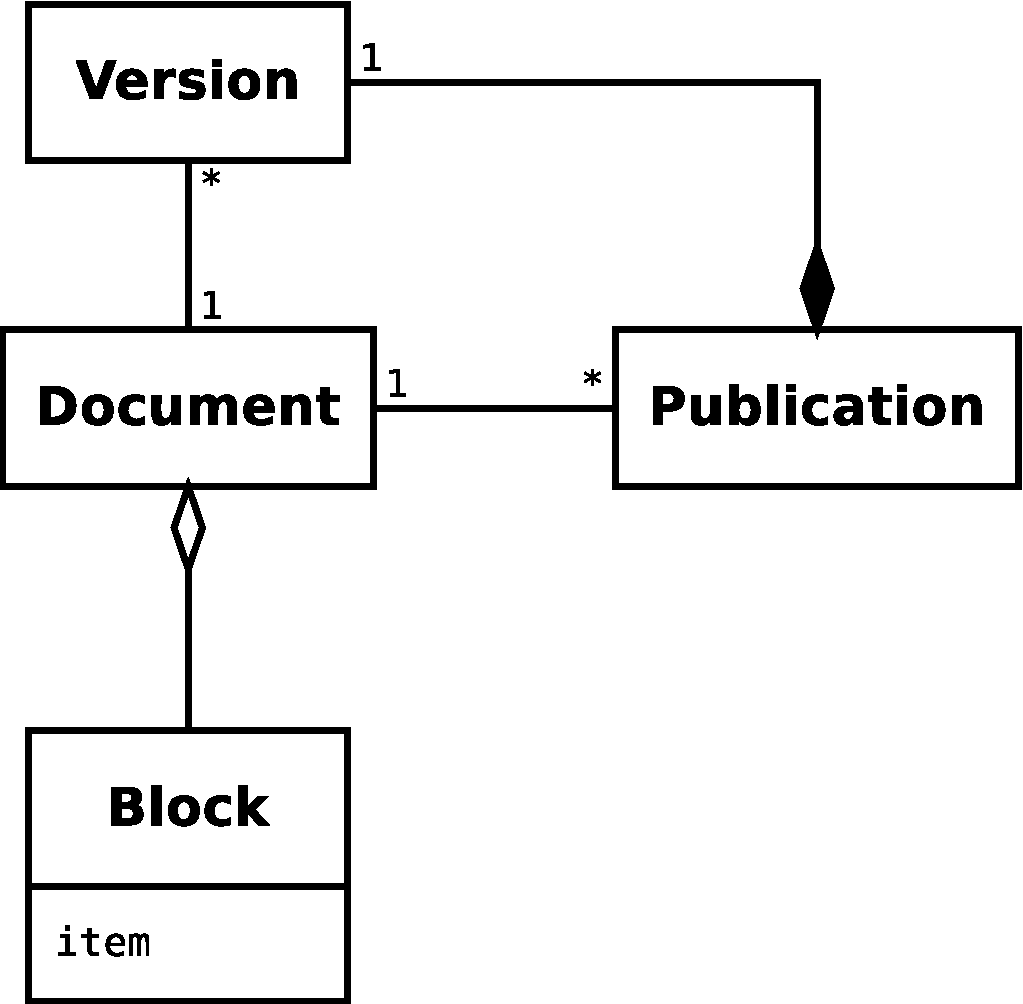
\includegraphics[width=75mm]{documents_conceptual.pdf}
  \caption{Conceptual Documents Model}
  \label{fig:documents_conceptual}
\end{figure}

\textbf{FIXME}

patterns used
\begin{itemize}
  \item \textsc{Memento} - used for versioning
  \item \textsc{Property} (simplified variant) - used for decoupling the type of the block item from the database schema
  \item pattern 3
\end{itemize}

The variant of the \textsc{Property} pattern implemented is simplified to the highly dynamic nature of the Ruby language --- which means that, for this particular problem, it is able to build new types of objects or even create new class definitions in runtime.

\subsection{Implementation}\label{sec:fa_documents_implementation}

\subsection{Impact Analysis}\label{sec:fa_documents_impact_analysis}
